\documentclass[12pt,a4paper]{scrreprt}
\usepackage[T1]{fontenc}
\usepackage[utf8]{inputenc}
\usepackage[ngerman]{babel}
\usepackage{babelbib}
\usepackage{parskip}
\usepackage{booktabs}
\usepackage{multirow}
\usepackage{subcaption}
\usepackage{microtype}
\usepackage{amsmath}
\usepackage{listings}
\usepackage{graphicx} % Zum Einbinden von Grafiken
\usepackage[dvipsnames]{xcolor}
\usepackage[colorlinks=true,linkcolor=Black,citecolor=MidnightBlue,urlcolor=MidnightBlue]{hyperref}
\usepackage{hyperref}
\usepackage{pgfplots} \pgfplotsset{compat=1.9}
\usepackage{helvet} % Schönere SansSerif-Schrift
\usepackage{times}  % Schönere Serif-Schrift
\usepackage[onehalfspacing]{setspace}

\pagestyle{headings}

\graphicspath{ {images/} } % Pfad-Prefix für einzubindende Grafiken. Es sind auch mehrere Pfade möglich, diese müssen jeweils in eigenen {Klammern} stehen.

\setkomafont{disposition}{\normalcolor\bfseries} % überall Serifen verwenden
% oder
%\renewcommand{\familydefault}{\sfdefault} % überall Sans-Serif verwenden

\lstset {
frame = single,
basicstyle=\small
}

% PDF-Optionen (werden in den Dateieigenschaften angezeigt)
\hypersetup{
pdftitle={Automatisches ausschneiden von Bildern aus Fotoalben},
pdfauthor={Mariella Dreißig, Tom Eckardt, Stefan Bergmann},
pdfsubject={Dokumentation Praktikum Bildverarbeitung},
pdfpagelayout=TwoColumnRight
}

%%% Eigene Makros
\newcommand{\qq}[1]{\glqq #1\grqq} % \qq{Text in Anführungszeichen}

\begin{document}
%%% Titelseite
\begin{titlepage}
\begin{center}
\LARGE Eberhard Karls Universität Tübingen\\
\large Mathematisch-Naturwissenschaftliche Fakultät \\
Wilhelm-Schickard-Institut für Informatik\\
[3cm]
\huge Dokumentation Praktikum Bildverarbeitung\\
[2cm]
\Large\textbf{Automatisches ausschneiden von Bildern aus Fotoalben}\\
[1.5cm]
\large Mariella Dreißig, Tom Eckardt, Stefan Bergmann\\
[0.5cm]
\today\\
\vfill
\small\textbf{Betreuer}\\[0.3cm]
\large Andreas Karge, Prof. Andreas Schilling\\
\end{center}
\end{titlepage}

%%% Titelrückseite: Bibliographische Angaben
\thispagestyle{empty}
\vspace*{\fill}
\textbf{Mariella Dreißig, Tom Eckardt, Stefan Bergmann:}\\
\emph{Automatisches ausschneiden von Bildern aus Fotoalben}\\
Dokumentation Praktikum Bildverarbeitung \\
Eberhard Karls Universität Tübingen\\
\newpage


%%% Zusammenfassung (Abstract), hier aus externer Datei eingebunden
\begin{abstract}
\section*{Zusammenfassung}
Das hier entwickelte Kommandozeilenprogramm extrahiert Bilder aus einer eingescannten Fotoalbumseite und kann Gesichter detektieren. Zum extrahieren wird der Floodfill-Algorithmus verwendet, der anhand der Hintergrundfarbe des Fotoalbums die Bilder ausschneidet. Um noch einen vorhandene Rahmen zu entfernen werden die Kanten des Bildes mit dem Canny-Algorithmus detektiert und an den Seiten des Bildes nach einem Bereich gesucht an dem keine Kanten sind. Danach kann mit Hilfe eines Cascade Classifier Gesichter in den Bildern detektiert werden. Dies geschieht sowohl für Gesichter im Profil als auch für Gesichter die direkt in die Kamera schauen. Um die Ergebnisse zu überprüfen werden die Bilder auf Größe, Featureposition und Strukturelle Ähnlichkeit hin überprüft. Das Programm arbeitet sehr gut bei Bildern mit einem deutlichen Rahmen und die gerade in der Seite ausgerichtet sind. Bilder deren Farbwerte stark dem Hintergrund ähneln oder die sich schräg in dem Fotoalbum befinden werden schlecht ausgeschnitten. Für die Gesichtserkennung ist die Qualität und Auflösung der Bilder ausschlaggebend. Bei schlechter Qualität werden wesentlich weniger Gesichter erkannt als bei Bilder mit guter Qualität.
\end{abstract}

\newpage

%%% Inhaltsverzeichnis
\KOMAoption{toc}{listof,bib} % Abbildungs-/Tabellenverzeichnis, Literaturverzeichnis aufnehmen
\tableofcontents\label{toc}
\cleardoublepage

%%% Hauptteil (mit \input{dateiname} wird die Datei 'dateiname' eingebunden)
\chapter{Einleitung}

% problemstellung
% ziele definieren
% vorhandene daten beschreiben
\section{Problemstellung}

\section{Benutzte Technologien}
% genutzte methoden, toolboxen, programmiersprachen

\section{Programmaufbau}

\cleardoublepage

\chapter{Hintergrundentfernung}
% Extraktion von Bildern aus einem monotonen Hintergrund
\cleardoublepage

\chapter{Extraktion eines Bildes aus einem monotonen Rahmen}
\cleardoublepage

\chapter{Gesichtserkennung}
% 2D BV, Machine Learning -> viola-jones-methode (haar-wavelets)
% opencv Funktionsweise (Dokumentation)
% frontal, profile
% probleme, Ergebnisse
Die Aufgabenstellung beinhaltet, in den extrahierten Fotos Gesichter zu erkennen. Hier muss die Gesichtserkennung (in der Fachliteratur "Face Detection") von der Wiedererkennung von bereits identifizierten Gesichtern (in der Fachliteratur "Face Recognition") unterschieden werden. In der vorliegenden Arbeit geht es ausschließlich darum, die Position von Gesichtern in den eingescannten Fotos zu erkennen und nicht, bereits erkannte Gesichter wiederzuerkennen oder zuzuordnen \footnote{Aufgrund der geringen Datenmenge und der schlechten Qualität der alten Fotos ist es nicht möglich, Gesichter wiederzuerkennen.}.\\
In der klassischen Bildverarbeitung wurden lange einfache 2D-Verfahren verwendet, um Gesichter in Bildern zu erkennen (\cite{Kees2012}, \cite{Wachter2001}). Beim Template Matching werden beispielsweise Vorlagen (von Teilen) von Gesichtern erzeugt um diese dann im Anwendungsfall mit den Zielbildern zu vergleichen. Dieses Verfahren ist nicht sehr robust, besonders bei sich verändernden Lichtverhältnissen, aber gleichzeitig extrem rechenaufwändig. \\
Eine einfachere Methode der Gesichtserkennung in der klassischen Bildverarbeitung ist die Nutzung von geometrischen Merkmalen in den Gesichtern. Hierbei werden beispielsweise Grauwerte in einem bestimmten Bereich des Bildes aufsummiert oder Gradientenoperatoren zur horizontalen und vertikalen Kantenerkennung angewandt. So kann die Ausrichtung, die relative Lage und ähnliche Merkmale der Nase, der Augen und des Munden identifiziert und zusammen als Gesicht klassifiziert werden. \\
Doch auch diese Methode ist rechen- und zeitintensiv. Deswegen wird häufig eher auf komplexere Methoden zur Gesichtserkennung gesetzt, wie beispielsweise das Elastic Bunch Graph Matching, das eine robuste Waveletanalyse nutzt (\cite{Wiskott1999}) oder die auf der Hauptkomponentenanalyse basierende Eigenfaces-Methode (\cite{doi:10.1162/jocn.1991.3.1.71}). Weiterentwicklungen dieser beiden Methoden werden heute noch eingesetzt, obwohl die Ansätze schon vergleichsweise alt sind. \\
Im Folgenden wird ein populärer Ansatz vorgestellt, der in den vorliegenden Arbeit verwendet wurde. 

\section{Cascade Classifier}
Die OpenCV Programmbibliothek beinhaltet vorimplementierte Funktionen zur Gesichtserkennung. Sie basiert auf einem 2001 entwickelten Ansatz zur Objekterkennung in Bildern (\cite{Viola2001}, \cite{Lienhart2002}). Es ist ein trainierter Classifier, der einfache geometrische Merkmale im Bild erkennt und auf deren Basis die gewünschten Objekte erkennen kann (\cite{OpenCV}).\\
Die Methode nutzt sogenannte Haar-ähnliche Features, mit denen grundlegende Strukturen (Helligkeitsunterschiede) im Bild erkannt werden. Im Bild \ref{fig:haarfeatures} werden alle Features aufgelistet, die der Classifier nutzen kann. Für die Gesichtserkennung werden in der Praxis aber nicht so viele genutzt, sondern nur einige wenige. Mit diesen können allgemeine Eigenschaften von menschlichen Gesichtern repräsentiert werden. So ist zum Beispiel die Nase heller als die Bereiche um die Augen, das entspricht dem Feature 2(a) in Bild \ref{fig:haarfeatures}.\\
\begin{figure}
	\centering
	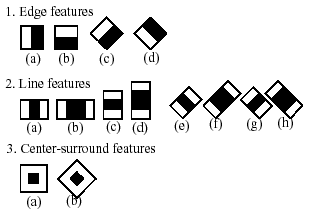
\includegraphics[width=0.5\linewidth]{images/haarfeatures.png}
	\caption{Alle vom Cascade Classifier Algorithmus genutzten Haar-ähnlichen Features zur Objekterkennung. Zur Gesichtserkennung werden nur fünf Features genutzt: 1(a), 1(b), 2(a), 2(c) und eine Kombination aus zwei 1(a) Features, die zusammen ein schachbrettartiges Muster ergeben.}
	\label{fig:haarfeatures}
\end{figure}
Nachdem die zu nutzenden Features ausgewählt wurden, wird ein Integralbild erzeugt, das in der Lage ist, die Features in konstanter Zeit auszuwerten. Dadruch wird eine relativ geringe Laufzeit erzielt.\\
In der Trainingsphase wird der Classifier mit Positiv- und Negativbeispielen von dem zu erkennenden Objekt trainiert, in diesem Fall mit Gesichtern \footnote{In der OpenCV Bibliothek ist sowohl ein Trainer als auch ein Detector enthalten. Der Detector ist vortrainiert kann direkt zur Gesichtserkennung verwendet werden. Wenn man genug Daten zur Verfügung hat, kann man aber auch einen selbst trainieren.}. Dieser Vorgang wird mit verschiedenen Arten des AdaBoostings beschleunigt und verbessert. Dadurch werden die besten Features für die Klassifizierung identifiziert. \\
Danach wird der Classifier in mehreren Stufen auf die Bilder angewandt ("cascade"), in denen das Objekt identifiziert werden soll. Jeder Classifier funktioniert dabei wie ein Filter, der die negativen Regionen aus dem Bild herausfiltert. Die verbleibenden Bereiche werden Stück für Stück durch immer komplexere Classifier gegeben, bis sie entweder aussortiert werden oder das Objekt (ein Gesicht) identifiziert wurde. Somit hat der Cascade Classifier die Struktur eines Entscheidungsbaumes und Rechenzeit wird gespart. Die Methode ist so robust, dass das Objekt in verschiedenen Größen in dem Bild erkennen kann, unabhängig von der Größe der Bilder, mit der der Classifier trainiert wurde.\\
Wenn die OpenCV Methode \texttt{detectMultiScale} ein Gesicht im Input-Bild erkennt, gibt es die Position in x- und y-Koordinaten und dessen Abmessungen (Höhe, Breite) zurück. In dem vorliegenden Programm werden zwei verschiedene Classifier auf die Bilder angewandt: einmal frontale Gesichter und einmal Gesichter im Profil. Die Rückgabewerte der Funktionen werden dafür genutzt, die Gesichter auszuschneiden und Dopplungen zu erkennen.
% nutzung in der praxis: https://docs.opencv.org/3.4/d7/d8b/tutorial_py_face_detection.html
\newpage

\chapter{Auswertung}

\section{Metriken zur Auswertung}
\subsection{Bildgröße}
Da es in dem Projekt um das Ausschneiden von Bildern geht ist die Bildgröße eine nahe liegende Metrik um die Genauigkeit unserer Software zu messen. Die Größe wird berechnet indem die Höhe mit der Breite multipliziert wird. Von der so ermittelten Größe des ausgeschnittenen Bildes wird die Größe des Ground Truth Bildes abgezogen. Aus dieser Differenz wird der Prozentuale unterschied zum Ground Truth Bild berechnet. Sollte das Ergebnis negativ sein ist das ausgeschnittene Bild kleiner als der Ground Truth.
   
\subsection{Bildmerkmale}
Eine weitere Metrik ist das erkennen gleicher Bildmerkmale. Dazu wird der patent freie ORB (Orientatet FAST and Rotated BRIEF) detektor von OpenCV verwendet der Rotations invariant ist. ORB ist eine fusion zwischen dem FAST Schlüsselpunkt Detektor and BRIEF Beschreibung der Schlüsselpunkte mit vielen Modifikationen um die Geschwindigkeit des Algorithmus zu verbessern (\cite{OpenCVORB}). Die so erkannten Merkmale werden dann der reihe nach anhand der Distanz zum Bildzentrum verglichen. Es wird für jedes erkannte Bildmerkmal die Distanz zum Zentrum des dazu gehörigen Bildes berechnet und das dann mit den Ergebnissen des Ground Truth verglichen. Solange zwischen den beiden Merkmalen keine zu großer Unterschied in der Distanz ist werden sie als gleich angesehen. Durch dieses Verfahren kann erkannt werden das sich der Ausschnitt des ausgeschnittenen Bildes an der selben stelle befindet, wie der Ground Truth und nicht nur die gleiche Größe ausgeschnitten wurde.

\subsection{Struktureller Ähnlichkeit (SSIM)}
Um ein Bild auf Gleichheit zu untersuchen verwenden wir den Strukturellen Ähnlichkeitsindex (Structural Similarity index, SSIM). Dieser berechnet die Ähnlichkeit zwischen verschiedenen Bildausschnitten mit folgender Gleichung:
$$
SSIM(x,y) = \frac{(2 \mu_x \mu_y + c_1)(\sigma_{xy} + c_2)}{(\mu^2_x + \mu^2_y + c_1)(\sigma^2_x + \sigma^2_y + c_2)}
$$ 
mit $\mu$ als Durchschnitt und $\sigma$ als Varianz bzw. Kovarianzmatrix des Bildausschnittes. $c$ sind da um die Division zu stabilisieren (\cite{Wang2004}). Das Verfahren lässt sich nur auf gleich große Bilder anwenden. Aus diesem Grund verkleinern wir die Bilder mit einer linearen Interpolation auf eine Größe von 64 x 64 Pixeln. Auf die so verkleinerten Bilder wird dann der SSIM angewandt. Um so näher das Ergebnis an 1 ist um so ähnlicher sind die beiden Bilder. 

\section{Ausgeschnittene Bilder}
In der Tabelle \ref{tab:metrics} sind die Ergebnisse für einige der Testbilder dargestellte den direkten Vergleich kann man in Abbildung ?? sehen dort sind die Bilder nebeneinander aufgezeigt. 

\begin{table}[h]
	\centering
	\begin{tabular}{c|ccc}
	Bild & Größe & Merkmale & SSIM \\ \hline 
	01 & 1.92 & 3.64 & 0.82 \\
	02 & 1.60 & 2.39 & 0.77 \\
	03 & -5.52 & 10.12 & 0.36 \\
	04 & 3.15 & 16.54 & 0.68 \\ 
	05 & 1.48 & 2.65 & 0.81 \\ \hline
	06 & -4.42 & 23.58 & 0.55 \\ 
	07 & 2.96 & 4.40 & 0.80 \\
	08 & 8.82 & 8.07 & 0.39 \\
	09 & -1.24 & 2.06 & 0.70 \\
	10 & -0.58 & 5.57 & 0.76 \\ \hline
	11 & -4.35 & 28.46 & 0.49 \\
	12 & 2.96 & 1.74 & 0.80 \\
	13 & 1.26 & 3.24 & 0.88 \\
	14 & 3.01 & 1.94 & 0.72 \\
	15 & 0.76 & 19.51 & 0.60 
	\end{tabular}
	\caption{Ergebnisse der Vergleichsmetriken der ausgeschnittenen Bilder.}
	\label{tab:metrics}
\end{table}


\section{Gesichtserkennung}
Die von OpenCV mitgelieferten Methoden zur Gesichtserkennung auf Bildern funktioniert grundsätzlich gut. Sie ist einfach anwendbar, hat eine vertretbare Laufzeit (der Algorithmus läuft nur einige Sekunden auf einer ganzen eingescannten Albumseite) und erkennt zumindest einen Großteil der Gesichter in den Fotos. \\
Um die Performanz der Classifier einzeln und in Kombination auszuwerten, wurden Wahrheitsmatrizen aufgestellt. Ausgewertet werden jeweils die korrekt erkannten Gesichter (True Positives (TP): positive - positive), die nicht erkannten Gesichter (False Negatives (FN): positive - negative) und die fälschlicherweise erkannten Gesichter (False Positives (FP): negative - positive). Korrekt nicht erkannte Gesichter (True Negatives (TN): negative - negative) gibt es in unserem Anwendungsfall nicht.\\
Tabellen \ref{tab:set1frontal} und \ref{tab:set2frontal} zeigen die Metriken in dem ersten und dem zweiten Datensatz wenn nur der frontal faces Classifier angewendet wird. Die daraus errechnete Genauigkeit \footnote{Formel für die Berechnung der Genauigkeit (\grqq Accuracy\grqq) ist: $\frac{TP + TN}{TP + FN + TN + FP}$, ($TN = 0$ in unserem Fall).} beträgt im ersten Datensatz 0.75 und im zweiten 0.59.\\
\begin{table}[h]
	\centering
	\begin{tabular}{l|lll}
		\hline
		& \multicolumn{3}{l}{Reference} \\ \hline
		\multirow{3}{*}{Prediction} &  & Positive & Negative \\
		& Positive & 270 & 1 \\
		& Negative & 88 & - \\ \hline 
	\end{tabular}
	\caption{Wahrheitsmatrix im ersten Datensatz, wenn nur der frontal-Classifier zum Einsatz kommt. Die Genauigkeit der Gesichtserkennung beträgt 0.75.}
	\label{tab:set1frontal}
\end{table}
\begin{table}[h]
	\centering
	\begin{tabular}{llll}
		\hline
		& \multicolumn{3}{l}{Reference} \\ \hline
		\multirow{3}{*}{Prediction} &  & Positive & Negative \\
		& Positive & 282 & 7 \\
		& Negative & 172 & - \\ \cline{2-4} 
	\end{tabular}
	\caption{Wahrheitsmatrix im zweiten Datensatz, wenn nur der frontal-Classifier zum Einsatz kommt. Die Genauigkeit der Gesichtserkennung beträgt 0.59.}
	\label{tab:set2frontal}
\end{table}
Wenn der zweite Classifier zur Erkennung von Profilen mit dazu genommen wird, erhöht sich die Anzahl der erkannten Gesichtern ein wenig. Das ist in Tabellen \ref{tab:set1frontalprofile} und \ref{tab:set2frontalprofile} zu sehen. Die Gesichter, die bereits von dem frontal-Classifier erkannt wurden, werden automatisch heraus gefiltert. Danach bleibt ein kleiner Mehrgewinn durch die Anwendung des profile-Classifiers übrig, die Performanz verbessert sich auf 0.76 und 0.65 jeweils.
\begin{table}[h]
	\centering
	\begin{tabular}{llll}
		\hline
		& \multicolumn{3}{l}{Reference} \\ \hline
		\multirow{3}{*}{Prediction} &  & Positive & Negative \\
		& Positive & 274 & 2 \\
		& Negative & 84 & - \\ \cline{2-4} 
	\end{tabular}
	\caption{Wahrheitsmatrix im ersten Datensatz, wenn frontal- und profile-Classifier kombiniert werden. Die Genauigkeit der Gesichtserkennung beträgt 0.76.}
	\label{tab:set1frontalprofile}
\end{table}
\begin{table}[h]
	\centering
	\begin{tabular}{llll}
		\hline
		& \multicolumn{3}{l}{Reference} \\ \hline
		\multirow{3}{*}{Prediction} &  & Positive & Negative \\
		& Positive & 301 & 8 \\
		& Negative & 153 & - \\ \cline{2-4} 
	\end{tabular}
	\caption{Wahrheitsmatrix im zweiten Datensatz, wenn frontal- und profile-Classifier kombiniert werden. Die Genauigkeit der Gesichtserkennung beträgt 0.65.}
	\label{tab:set2frontalprofile}
\end{table}

\subsubsection*{Festlegung der Ground Truth}
Die Referenz für die Auswertung der Gesichtserkennung festzulegen ist nicht trivial. Auf den alten Fotos sind aufgrund der schlechten Qualität der Aufnahmen viele Gesichter nicht tatsächlich zu erkennen. Vielmehr erschließt sich ein menschlicher Betrachter aus dem Kontext die Information, dass sich an gewissen Stellen ein Gesicht befinden muss. Das wurde bei der Festlegung der Ground Truth berücksichtigt. So wurden beispielsweise besonders kleine, verdeckte oder stark verschwommene Gesichter für die Berechnung der Metriken nicht berücksichtigt. Die Classifier haben außerdem Probleme, Gesichter zu erkennen, wenn starke Okklusionen auftreten, selbst wenn das Gesicht nur im Profil zu erkennen ist oder die Person eine Kopfbedeckung trägt. Diese wiederum wurden in die Gesamtsumme der Gesichter mit einberechnet. Im Folgenden werden exemplarisch einige Bilder gezeigt, die der Gesichtserkennungsalgorithmus nicht erkennen kann und die deswegen nicht in die Auswertung mit einbezogen wurden.\\
Bild \ref{fig:neg_ex1} zeigt ein kleines Mädchen, jedoch ist die Aufnahme sehr verschwommen. Jeder Mensch, der das Bild betrachtet, weiß, dass das Mädchen ein Gesicht haben muss. Wenn jedoch die Kontextinformationen entfernt werden würde, wäre es selbst für einen Menschen schwer, ein Gesicht zu identifizieren.\\
\begin{figure}[h]
	\centering
	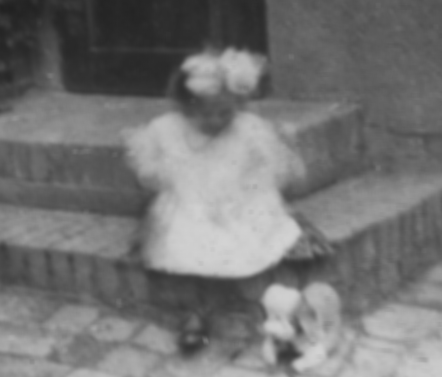
\includegraphics[width=0.75\linewidth]{images/examples_groundtruth/negative/04_1.png}
	\caption{Starke Bewegung im Bild verhindert, dass das Gesicht des Mädchens tatsächlich zu sehen ist, auch wenn menschliche Betrachter durchaus ihr Gesicht erkennen könnten.}
	\label{fig:neg_ex1}
\end{figure}
Auf Bild \ref{fig:neg_ex2} ist eine ähnliche Situationen zu sehen: alle abgebildeten Menschen haben Gesichter, jedoch sind sie objektiv nicht wirklich zu sehen. Sie sind relativ klein, was normalerweise für den Classifier kein Problem darstellt, aber eine schlechte Beleuchtung und geringer Kontrast tragen dazu bei, dass die Gesichter nicht erkannt werden.\\
\begin{figure}[h]
	\centering
	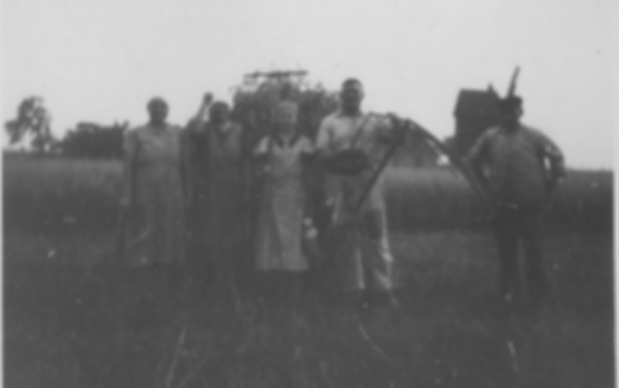
\includegraphics[width=0.75\linewidth]{images/examples_groundtruth/negative/29_2.png}
	\caption{Die Gesichtserkennung schlägt fehlt, wenn die Gesichter zu schlecht beleuchtet sind und/oder zu wenig Kontrast aufweisen. Auch, wenn normalerweise auch Gesichter in dieser Größe von dem Algorithmus problemlos erkannt werden.}
	\label{fig:neg_ex2}
\end{figure}
Um dennoch eine repräsentative Auswertung der Performanz der Gesichtserkennung zu gewährleisten, wurden viele nicht erkannte Gesichter mit in die Metriken einberechnet. Beispielsweise können die Classifier keine Gesichter mit Kopfbedeckungen erkennen. Ansonsten sind aber die Gesichter gut zu identifizieren, was in Bild \ref{fig:pos_ex1} zu sehen ist.\\
\begin{figure}[h]
	\centering
	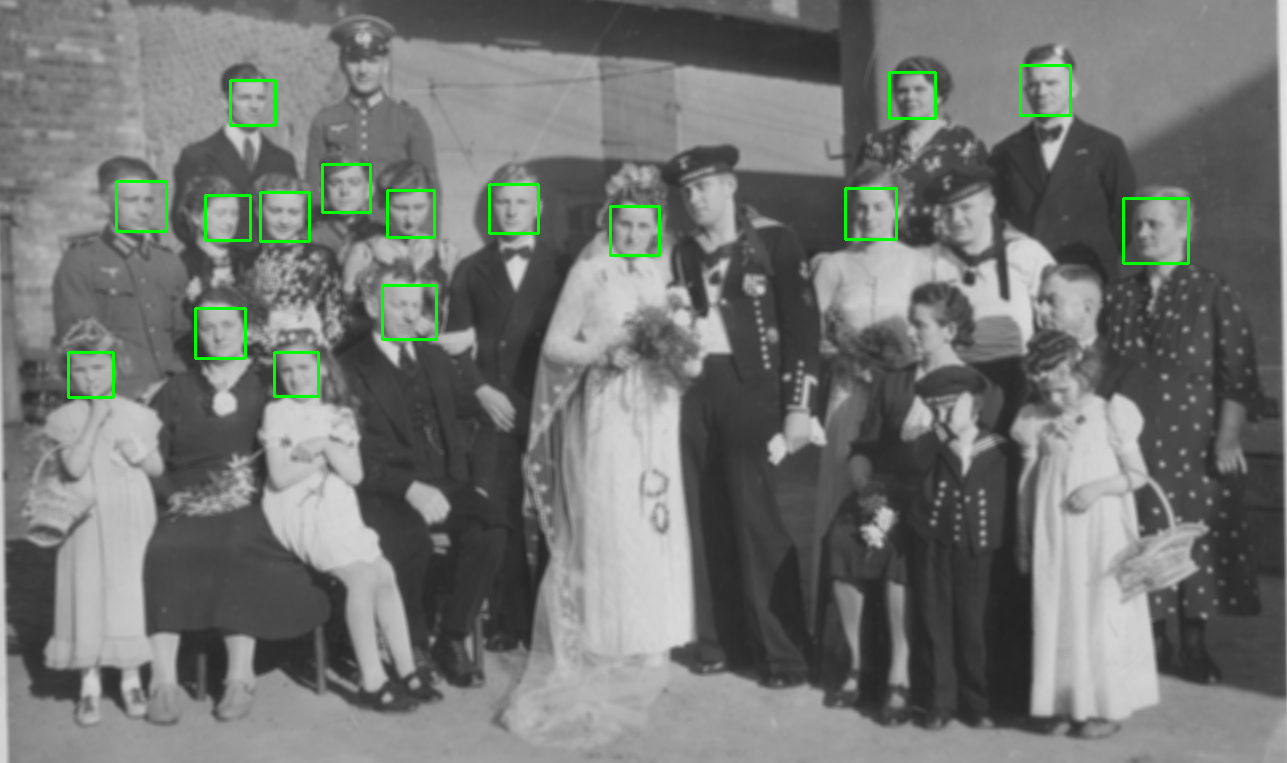
\includegraphics[width=0.75\linewidth]{images/examples_groundtruth/positive/32_3.png}
	\caption{Kein Classifier erkennt Gesichter mit Hüten, auch wenn sie nur einen kleinen Teil vom Gesicht verdecken. Alle anderen Gesichter werden problemlos identifiziert.}
	\label{fig:pos_ex1}
\end{figure}
Bild \ref{fig:pos_ex2} zeigt einen problematischen Grenzfall aus dem zweiten Datensatz. In diesem Bild wurden insgesamt drei Gesichter erkannt (zwei vom frontal-Classifier (grün) und eins vom profile-Classifier (rot)). Da alle Gesichter in etwa die gleiche Größe und Schärfe haben, sollte angenommen werden, dass auch die restlichen Personen erkannt werden. Es ist nicht ersichtlich, warum auf diesem Bild beide Classifier keine weiteren Gesichter erkennen. Von daher fließen alle Gesichter auf diesem Foto mit in die Bewertung ein und erhöhen die Anzahl der False Negatives enorm. Besonders im zweiten Datensatz kommen solche Fälle häufiger vor, was die schlechte Performanz des Algorithmus' im Vergleich zum ersten Datensatz erklärt.
\begin{figure}[h]
	\centering
	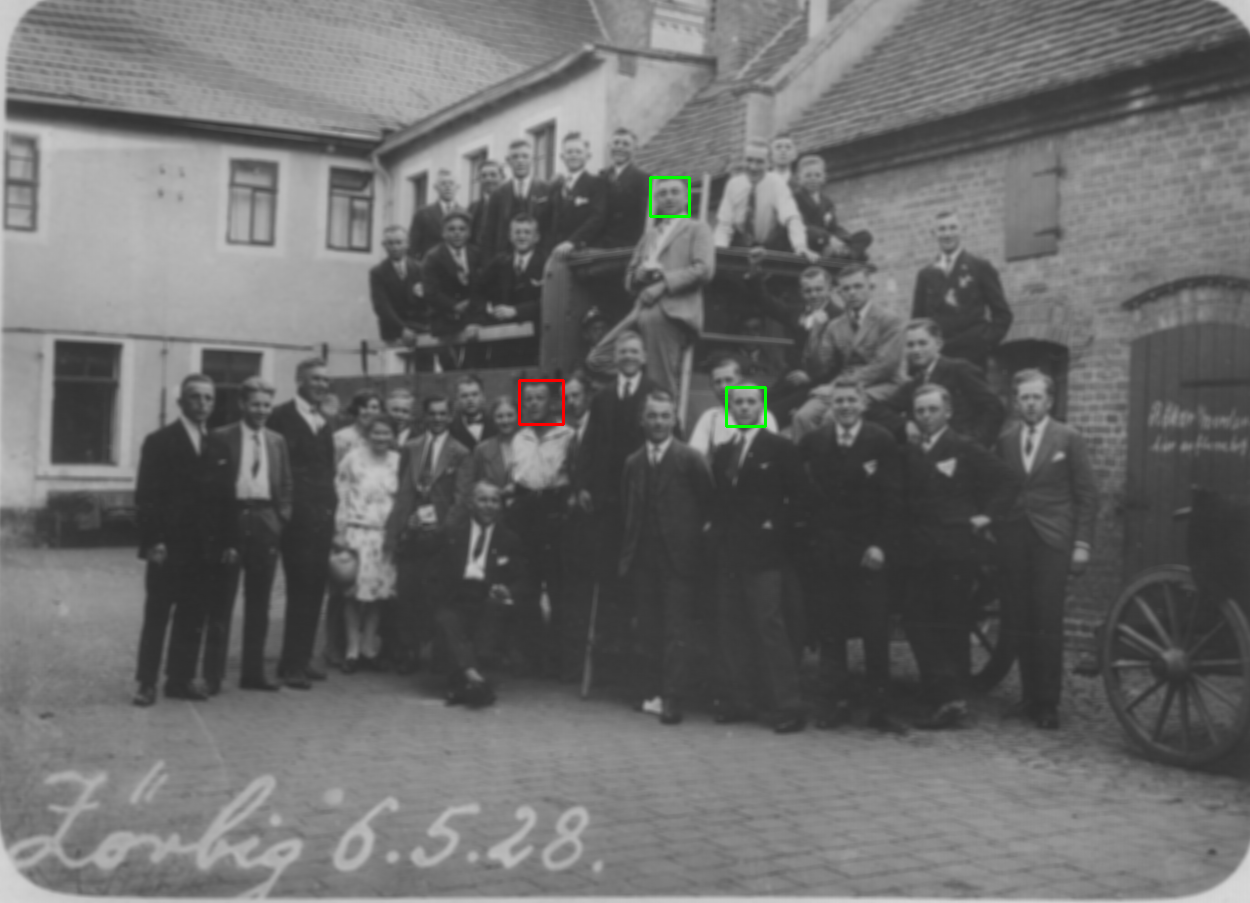
\includegraphics[width=0.75\linewidth]{images/examples_groundtruth/positive/16_1.png}
	\caption{In diesem Gruppenfoto werden nur wenige Gesichter erkannt, obwohl sie alle ähnlich aussehen. Das verschlechtert die Kennwerte für die Genauigkeit besonders im zweiten Datensatz stark.}
	\label{fig:pos_ex2}
\end{figure}
\cleardoublepage

\chapter{Fazit}
\cleardoublepage

\chapter{Benutzung und Konfiguration}
% workflow
% parameterbeschreibung
\cleardoublepage

%%% Literaturverzeichnis, lädt die Datei literatur.bib
\bibliographystyle{babplain} % "babplain" benötigt das Paket babelbib
\bibliography{literatur}
\cleardoublepage

\end{document}